\chapter{Realisierung}
% TODO Beschreibung der Umsetzung der definierten Ziele, einschliesslich der aufgetretenen Schwierigkeiten und Einschränkungen

% Dies ist das Hauptkapitel Ihrer Arbeit! Hier wird die Umsetzung der eigenen Ideen und Konzepte
% (Kapitel 3) anhand der gewählten Methoden (Kapitel 4) beschrieben, inkl. der dabei aufgetretenen
% Schwierigkeiten und Einschränkungen.

\section{Projektmanagement}

\subsection{Resultate}

Die folgende Tabelle~\fullref{tab:resultate} beschreibt alle Resultate und Unterresultate die während dieser Bachelorarbeit erstellt werden.
Diese Tabelle wurde zusammengestellt anhand der Anforderungen im Abschnitt~\ref{sec:Anforderungen}.

Jedes Resultat hat einen eindeutigen Identifier in  der Spalte ''Nr'' aufgelistet.
Die Spalte ``Anforderung'' bezieht sich darauf, welche Anforderungen für das jeweilige Resultat massgebend sind.
In der letzten Spalte ''Geschätzter Arbeitsaufwand'', wurde zu beginn des Projekts abgeschätzt wie viel Arbeitsaufwand (in Stunden) das Resultat verursacht.

\begin{longtable}{p{0.8cm} l p{3.5cm} p{2cm}}
    \toprule
    \bfseries Nr & \bfseries Resultat & \bfseries Anforderung& \multicolumn{1}{p{3cm}}{\bfseries Geschätzter Arbeitsaufwand} \\
    \midrule \endhead
    D            & \textbf{Dokumentation}                                       & \reqref{DOCS} & \textbf{Total 44h}  \\
    \midrule                                                               
    D.1          & \; Dokumenten Layout                                &       & 8h   \\
    D.2          & \; Aufbau des Berichts                              &       & 4h   \\
    D.3          & \; Titelseite                                       &       & 2h   \\
    D.4          & \; Zusammenfassung / Abstract                       &       & 2h   \\
    D.5          & \; Einleitung                                       &       & 4h   \\
    D.6          & \; Beschreibung Motivation / Problem                &       & 2h   \\
    D.7          & \; Beschreibung der Aufgabenstellung                &       & 2h   \\
    D.8          & \; Beschreibung der Ziele / Vision                  &       & 1h   \\
    D.9          & \; Fragestellungen / Hypothesen                     &       & 2h   \\
    D.11         & \; Reflektion / Fazit                               &       & 3h   \\
    D.12         & \; Persönliches Projektfazit                        &       & 1h   \\
    D.13         & \; Ausblick                                         &       & 4h   \\
    D.14         & \; Anhang                                           &       & 3h   \\
    D.15         & \; Zwischenpräsentation                             & \reqref{PRES}  & 6h  \\
    \midrule                                                               
    R            & \textbf{Research State of the Art}                           & \reqref{SDTF} \reqref{DOCS}  & \textbf{Total 40h} \\
    \midrule                                                               
    R.1          & \; Literatur sammeln (Recherche)                    &       & 12h  \\
    R.2          & \; Bibliographie erstellen                          &       &  4h  \\
    R.3          & \; P2P Networks                                     &       &  2h  \\
    R.3.1        & \;   - Latenz / Bandbreite / Performanz             &       &  2h  \\
    R.4          & \; Beschreibung I2P                                 &       & 10h  \\
    R.4.1        & \; -- Begrifflichkeiten                              &       &  4h  \\
    R.4.2        & \; -- Funktionsweise                                 &       &  2h  \\
    R.4.3        & \; -- Bandbreite                                     &       &  2h  \\
    R.4.4        & \; -- Latenz                                         &       &  2h  \\
    R.5          & \; Deployment von Testnetzwerken                    &       &  4h  \\
    R.6          & \; Beschreibung der Wissenschaftlichen Methode      &       &  2h  \\
    R.7          & \; Metriken für die Auswertung                      & \reqref{TPER} \reqref{TISO} \reqref{TREP}  &  6h  \\
    \midrule                                                               
    K            & \textbf{Testkonzept          }                               & \reqref{TKON} \reqref{DOCS}  & \textbf{Total 46h}  \\
    \midrule                                                               
    K.1          & \; Beschreibung Ideen / Konzepte                    &       &  4h  \\
    K.2          & \; Anforderungen an den Teststand                   &       &  4h  \\
    K.3          & \; Teststrategie                                    &       &  4h  \\
    K.4          & \; Architektur Teststand                            &       &  4h  \\
    K.5          & \; Komponentendiagramm                              &       &  2h  \\
    K.6          & \; Beschreibung was gemessen werden soll            &       &  8h  \\
    K.7.1        & \; -- Bandbreite                                     & \reqref{TLIM} &  2h  \\
    K.7.1        & \; -- Anzahl Tunnels                                 & \reqref{TCNF}    &  2h  \\
    K.7.1        & \; -- Latenz von Nachrichten                         & \reqref{TLAT}    &  2h  \\
    K.7.1        & \; -- Ressourcenauslastung eines Knotens             & \reqref{TPER}    &  2h  \\
    K.8          & \; Beschreibung wie gemessen wird                   &       & 10h  \\
    K.8.1        & \; -- Isolation des Netzwerks                        & \reqref{ORDR}    &  2h  \\
    K.8.1        & \; -- Verschiedene Netzwerksegmente                  & \reqref{ORDR}    &  2h  \\
    K.8.2        & \; -- Latenz                                         & \reqref{ORDR}    &  2h  \\
    K.8.3        & \; -- Bandbreite                                     &       &  2h  \\
    K.8.4        & \; -- Konfigurationsmöglichkeiten                    & \reqref{TCNF} &  2h  \\
    K.9.5        & \; \glsname{ci}                                     & \reqref{TVRS} &  6h  \\
    K.9.6        & \; Beschreibung der Auswertungsmethode              &               &  4h  \\
    \midrule                                                               
    S            & \textbf{Teststand Design und Implementation}                 & \reqref{TINF} \reqref{DOCS} & \textbf{Total 124h} \\
    \midrule
    S.1          & \; Software Design                                  &       &  16h \\
    S.1          & \; Implementation                                   &       &  72h \\
    S.2.1        & \; -- Deployment des Testnetzwerkes                  & \reqref{TVRS} \reqref{TPER} &  8h \\
    S.2.2        & \; -- Netzwerksegmentierung                          & \reqref{TISO} &  8h \\
    S.2.3        & \; -- Konfigurationsmöglichkeiten                    & \reqref{TCNF} &  8h \\
    S.2.4        & \; -- Skalierung                                     & \reqref{TSCL} &  8h \\
    S.2.5        & \; -- Bandbreitenbeschränkung                        & \reqref{TLIM} &  8h \\
    S.2.6        & \; -- Reproduzierbarkeit                             & \reqref{TREP} &  8h \\
    S.2.7        & \; -- Latenzmessung                                  & \reqref{TLAT} &  8h \\
    S.2.8        & \; -- Messung der Ressourcenauslastung               & \reqref{TPER} &  8h \\
    S.2.9        & \; -- Verschiedene Testaufbauten                     & \reqref{TVRS} &  8h \\
    S.3          & \; Test des Labors                                  &       &  24h \\
    S.4          & \; Handbuch für den Teststand                       &       &  12h \\
    S.4.1        & \; -- Installation                                   &       &   2h \\
    S.4.3        & \; -- Konfiguration                                  &       &   2h \\
    S.4.3        & \; -- Ausführen von Messungen                        &       &   2h \\
    S.4.3        & \; -- Beschreibung der gesammelten Messdaten         &       &   4h \\
    S.4.3        & \; -- Beispiele                                      &       &   2h \\
    \midrule                                                                        
    A            & \textbf{Messung und Auswertung}                              & \reqref{EVAL} \reqref{DOCS}   & \textbf{Total 52h}  \\
    \midrule
    A.1          & \; Sammlung an Messdaten für die Auswertung         &        &  12h  \\
    A.2          & \; Beschreibung der Auswertungsmethode              &        &   4h  \\
    A.3          & \; Auswertung der Messungen                         &                    & 20h  \\
    A.3.1        & \; -- Einfluss der Knoten auf die Latenz             & \reqref{TLAT}      &  6h  \\
    A.3.2        & \; -- Einfluss der Anzahl Verbindungen auf die Latenz& \reqref{TLAT} \reqref{TLIM} &  6h  \\
    A.3.3        & \; -- Einfluss der Bandbreite auf Latenz             & \reqref{TLAT} \reqref{TLIM} &  6h  \\
    A.3.4        & \; -- Äussere Einflüsse / Unreinheiten               & \reqref{TREP} \reqref{TISO} &  2h  \\
    A.4          & \; Verschiedene Diagramme/Grafiken                  &       &  8h  \\
    A.5          & \; Auswertung der Anforderungen an den Teststand    & \reqref{TINF} &  4h  \\
    A.6          & \; Zusammenfassung der Auswertung                   &       &  4h  \\
    \midrule                                                               
    P            & \textbf{Project Management Dokumentation}                    & \reqref{DOCS} \reqref{ITER}  &  \textbf{Total 54h}  \\
    \midrule
    P.1          & \; Beschreibung Projektorganisation                 &       &  1h  \\
    P.3          & \; Projektmanagement Methode                        &       &  2h  \\
    P.2          & \; Beschreibung Projektumfang                       &       &  2h  \\
    P.4          & \; Projektplanung                                   &       &  8h  \\
    P.5          & \; Liste von Requirements                           &       &  4h  \\
    P.6          & \; Liste von Resultaten                             &       &  4h  \\
    P.9          & \; Arbeitsjournal                                   &       &  4h  \\
    P.10         & \; Meeting-Protokolle und Notizen                   &       & 29h  \\
    \midrule                                                               
                 & \bfseries  Geschätzter Arbeitsaufwand               & \textbf{Total} & \bfseries 360h \\
    \midrule
    \bottomrule
    \caption{Resultate}
    \label{tab:resultate}
\end{longtable}

Diese Liste von Resultaten ist auch ein guter Ausgangspunkt um davon Issues für den Issue-Tracker zu erstellen.
Jeder issue kann nun auch sortiert werden nach Resultat-Kategorien z.B. ''Recherche'', ''Projektmanagement'', ''Dokumentation'', ''Evaluation'', ''Präsentation'', etc.

\newpage

\section{Systemarchitektur}

\section{Komponentendesign}


\subsection{Bootstrapping}

Es wird Boostrapping-Prozess benötigt, dass sich die I2P-Router sich anfangs Gegenseitig im privaten und abgeschotteten Testnetzwerk überhaupt finden können.
Erst anschliessend ist es möglich Tunnels aufzubauen, damie die I2P-Router miteinander kommunizieren können.

Die I2P-Router im öffentlichem I2P-Netzwerk können sich hier einfach an den öffentlich verfügbaren Reseeder eine \lstinline|su3|-Datei herunterladen.
Diese \lstinline|su3|-Datei beinhaltet RouterInfos. 
Diese RouterInfos beinhalten die nötigen Informationen wie public-key und Netzwerkadresse, um die Kommunikation zu starten.

Im privaten und abgeschotteten Testnetzwerk sind die öffentlichen Reseed-Server jedoch nicht erreichbar.
Deshalb muss ein anderer Weg gefunden werden das private I2P-Netzwerk zu bootstrappen.

Einerseits gibt es hier den Floodfill-Ansatz oder einen eigen Reseed-Server zu im privaten Testnetzwerk zu haben.
%TODO: reference bootstrapping site


Um bessere empirische Aussagen machen zu können, sollte das Testnetzwerk so gut wie möglich das öffentliche I2P-Netzwerk abbilden \seereq{EVAL}.

Denn der Floodfill-Anstatz entspricht nicht umbedingt der realität, denn die Reseeder-Knoten können liefern nicht allen I2P-Routern dieselbe Liste an Peers.

Auch kann die Konfiguration des Reseeders eine wichtige Rolle spielen, denn dieser bestimmt mit der Liste an Peers die er den I2P-Routern liefert den Konnektivitätsgrad der Knoten.


\subsection{Konfiguration}

Die Konfiguration des Teststands kann mittels einer json-Konfigurationsdatei einfach angepasst werden.
Diese kann, falls nötig einfach von verschiedenen Orten gelesen werden.

\subsection{Resultate zurücklesen}

Just read logs? Use some Docker cp magic?

\section{Umsetzung / Programmierung}

Der Quellcode für das Testnetzwerk ist im folgenden Repository zu finden:

\subsection{VM / Container Netzwerk}

NixOS erlaubt es deklarativ Container zu definieren.

% \begin{lstlisting*}[language=nix,label=src:nixos-container,caption=Beispiel wie Nixos Container definiert werden können]
%
%     boot.enableContainers = true;
%     containers = {
%         "container1" = {
%             config = { config, pkgs, ... }:
%                 {
%                     # NixOS system configuration for this container
%                     services.httpd.enable = true;
%                 }
%             # more container settings ... 
%         };
%         # "container2" .... 
%     }
% \end{lstlisting*}

Wichtig dabei ist, dass es sich hierbei nicht um einen Docker-Container, sondern um NixOS-Container handelt.
Im Hintergrund brauchen jedoch beide Container-Arten die gleichen Linux-Kernel-Features (namespaces, cgroups, ... ).


Siehe \lstinline|containers.nix| in der \lstinline|i2p-testnet| Repository für die Effektive implementation


\url{https://codeberg.org/mkuettel/i2p-testnet}.

\subsection{Bootstrapping}

\subsubsection{Reseed-Server}

Dieser Ansatz hat den Vorteil, das so das Testnetzwerk schnell aufgebaut werden kann.

Die \lstinline|i2pd|-Implementation beinhaltet selber keinen 

Die Go-Implementation dieses Reseed-Servers ist hier zu finden:

\url{https://codeberg.org/diva.exchange/i2p-tools}

Diese version basiert auf der folgenden GitHub version:

\url{https://github.com/MDrollette/i2p-tools}

\subsubsection{Ablauf}


Der Bootstrapping-Vorgang im Testnetzwerk wird wie folgt abgehandelt:

\begin{enumerate}
    \item Erstellen der Container für den Reseed-Sever und den I2P-Knoten
    \item Der Reseed-Server erstellt die nötigen Schlüssel und Zertifikate, um einerseits später den HTTPS-Reseed-Server zu starten und andererseits die su3-Dateien zu signieren.
    \item Der Reseed-Server-Container fängt an zu warten bis er alle RouterInfo's von allen I2P-Knoten erhalten hat
    \item Die I2P-Router werden kurzzeitig gestartet, bis diese Ihre RouterInfo Datei erstellen. Die I2P-Router werden anschliessend wieder gestoppt, da der Reseed-Server im Moment noch nicht in Betrieb ist, da ihm die RouterInfos noch fehlen.
    \item Die I2P-Knoten-Container warten anschliessend bis der HTTPS-Reseed-Server verfügbar ist.
    \item Auf der Test-VM kopiert ein Hintergrund-Job alle RouterInfos vom I2P-Container in die NetDb des Reseed-Server-Containers.
    \item Nach kurzer Zeit hat der Reseed-Server-Container alle benötigten RouterInfos. Nun generiert dieser die su3-Datei aus den RouterInfos und startet anschliessend nun effektiv den HTTPS-Reseed-Server.
    \item Die I2P-Knoten-Container können nun den HTTPS-Reseed-Server erreichen und somit wird der I2P-Router gestartet.
    \item Die I2P-Router laden nun die su3-Datei herunter und können so die anderen Knoten ausfindig machen und Ihre Arbeit starten.
\end{enumerate}

Welche Reseeder ein I2P-Router anfragt, kann mittels der \lstinline|i2pd|-Konfigurationsoption \lstinline|urls| festgelegt werden.


\clearpage
\begin{landscape}% Landscape page
\begin{figure*}[ht]
  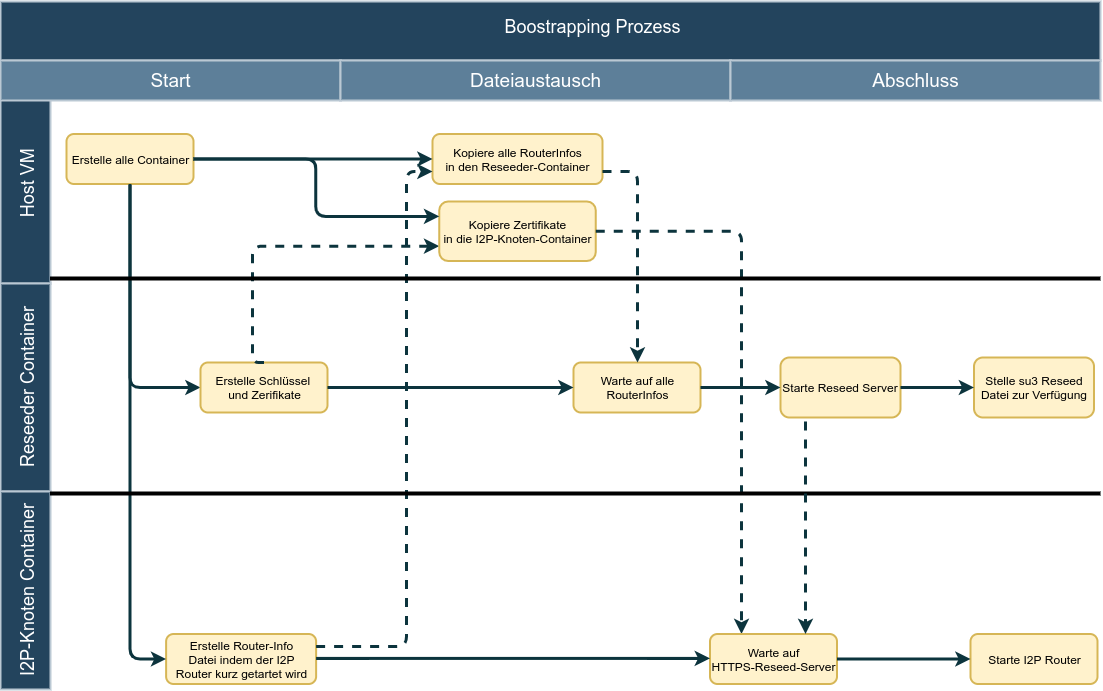
\includegraphics[height=0.85\textwidth]{bootstrap-diagram.png}
  \caption{Der Boostrapping Prozess}\label{fig:bootstrap-diagram}
\end{figure*}
\end{landscape}% Landscape page


\subsection{Reproduzierbarkeit}

* Nix
* Pinning
    
\cite{noauthor_nixops_nodate-5}


\subsection{Isolieren}

Während unserer Tests wollen wir nur Traffic unserer eigenen Knoten im Netzwerk 

docker-compose respektive docker hat die option ein eigenes Netzwerk zu erstellen:

\subsubsection{Abgrenzen vom Haupt-Netzwerk}

Die Konfigurationsoption \lstinline|netid| erlaubt es die Netzwerknummer zu definieren.
Beim realen I2P-Netzwerk ist diese standardmässig auf \lstinline|2| gesetzt.

VM / Container, Konfigurationsoption \lstinline|nat|

Nix für container scheint nicht so gut zu funktionieren

Weil:

Das Builder der systemkonfigurationen inkl. der container getestet mit 100 konnte nicht durchlaufen da nix viel memory braucht (ich habe nach 16GB und 20min warten aufgehört da mein Laptop am swappen war)
Fehlerhafte netzwerkkonfiguration by default, falsche routen und ip konfigurationen (fehlende definition der netzwerkmaske)
Container selber sind unnötig gross

\section{Testing}

CI? most don't allow this...

have a machine to deploy to

\section{Benutzerhandbuch}


